\documentclass[a4paper, 12pt]{article}
% math symbols
\usepackage{amssymb}
\usepackage{amsmath}
\usepackage{mathrsfs}
\usepackage{physsummer}


\usepackage{enumitem}
\usepackage[margin = 2cm]{geometry}

\tolerance = 1000
\emergencystretch = 0.74cm



\pagestyle{empty}
\parindent = 0mm

\begin{document}

\begin{center}
  \Large{\textbf{Городской центр физического образования, 10 класс.}\\
  \textit{Серия 7Ш, 10 ноября 2014.}}
\end{center}

\begin{center}
  \Large\textbf{ Районный тур уже близко. }
\end{center}

\large


\task{ В калориметре со льдом находится резистор. Сопротивление
  резистора зависит от температуры $T$, измеряемой в градусах Цельсия,
  по закону: $R(T) = R_0 + \chi T$, где $R_0$ и $\chi$~---~постоянные
  величины. Резистор подключают к источнику постоянного напряжения
  $U$. Определите зависимость температуры содержимого калориметра от
  времени вплоть до момента, когда температура станет равна $T_{\ast}$
  ($0^{\circ}C < T_{\ast} < 100^{\circ}C$). Постройте график
  полученной зависимости. Масса льда равна $m$, начальная температура
  $0^{\circ}C$. Удельная теплоёмкость плавления льда равна $\lambda$,
  удельная теплоёмкость воды $c$. Теплопотерями и теплоёмкостью
  резистора пренебречь. Считайте, что содержимое калориметра
  перемешивается и всё время находится в состоянии теплового
  равновесия. }
% СПб, район-10, 2013

\taskpic{ В прямоугольной комнате есть одно окно \textbf{W} и две
  отопительные батареи \textbf{B1} и \textbf{B2}. Первая батарея
  находится под окном, вторая — у противоположной стенки. Мощность
  первой батареи равна $W_1=1.2$ кВт, а второй $W_2 = 1$ кВт. Мощность
  батареи не зависит от температуры окружающей среды. Окно пропускает
  тепло. Коэффициент теплопередачи окна равен $k_1=110\mbox{
    Вт}/{}^{\circ} C$: это означает, что мощность потока тепла через
  окно равна $P=k_1 (T_1 - T_2)$, где $T_{1,2}$ — температуры с двух
  сторон от окна. Комнату разделили пополам ширмой \textbf{S} с
  коэффициентом теплопередачи равным $k_2=200\mbox{ Вт}/{}^{\circ}
  C$. Какая температура установится после этого в правой части
  комнаты? Температура на улице $0^{\circ}C$. Прочими теплопотерями
  пренебречь. }
{
  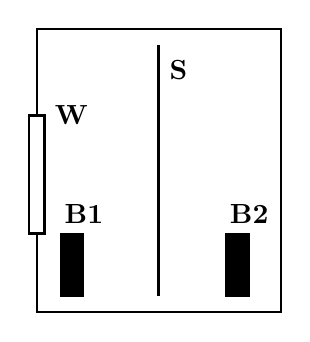
\begin{tikzpicture}
    \draw[thick] (0.5,0) rectangle (3.6,3.6);
    \draw[thick,fill=white] (0.4,1) rectangle (0.6,2.5) node[right]
    {\textbf{W}};
    \draw[fill=black] (0.8,0.2) rectangle (1.1,1) node[above]
    {\textbf{B1}};
    \draw[fill=black] (2.9,0.2) rectangle (3.2,1) node[above]
    {\textbf{B2}};
    \draw[very thick] (2.05,0.2) -- (2.05,3.4) node[right,pos=0.9] {\textbf{S}}; 
  \end{tikzpicture}
}
% СПб район-10, 2012

\task{ Десантник массой $m$ спускается с вертолёта на землю по тросу с
  постоянной относительно земли скоростью $v$. Трос невесомый и
  упругий, его жёсткость равна $k$, длина в нерастянутом состоянии
  $L$. Какая тепловая мощность выделяется за счёт трения десантника о
  трос? Ускорение свободного падения равно $g$. } 
% СПб район-10, 2014


\end{document}


%%% Local Variables: 
%%% mode: latex
%%% TeX-engine:xetex
%%% TeX-PDF-mode: t
%%% End:
